The best performing network is reported in Figure \ref{fig:reg_net}.
\begin{figure}[h]
    \centering
    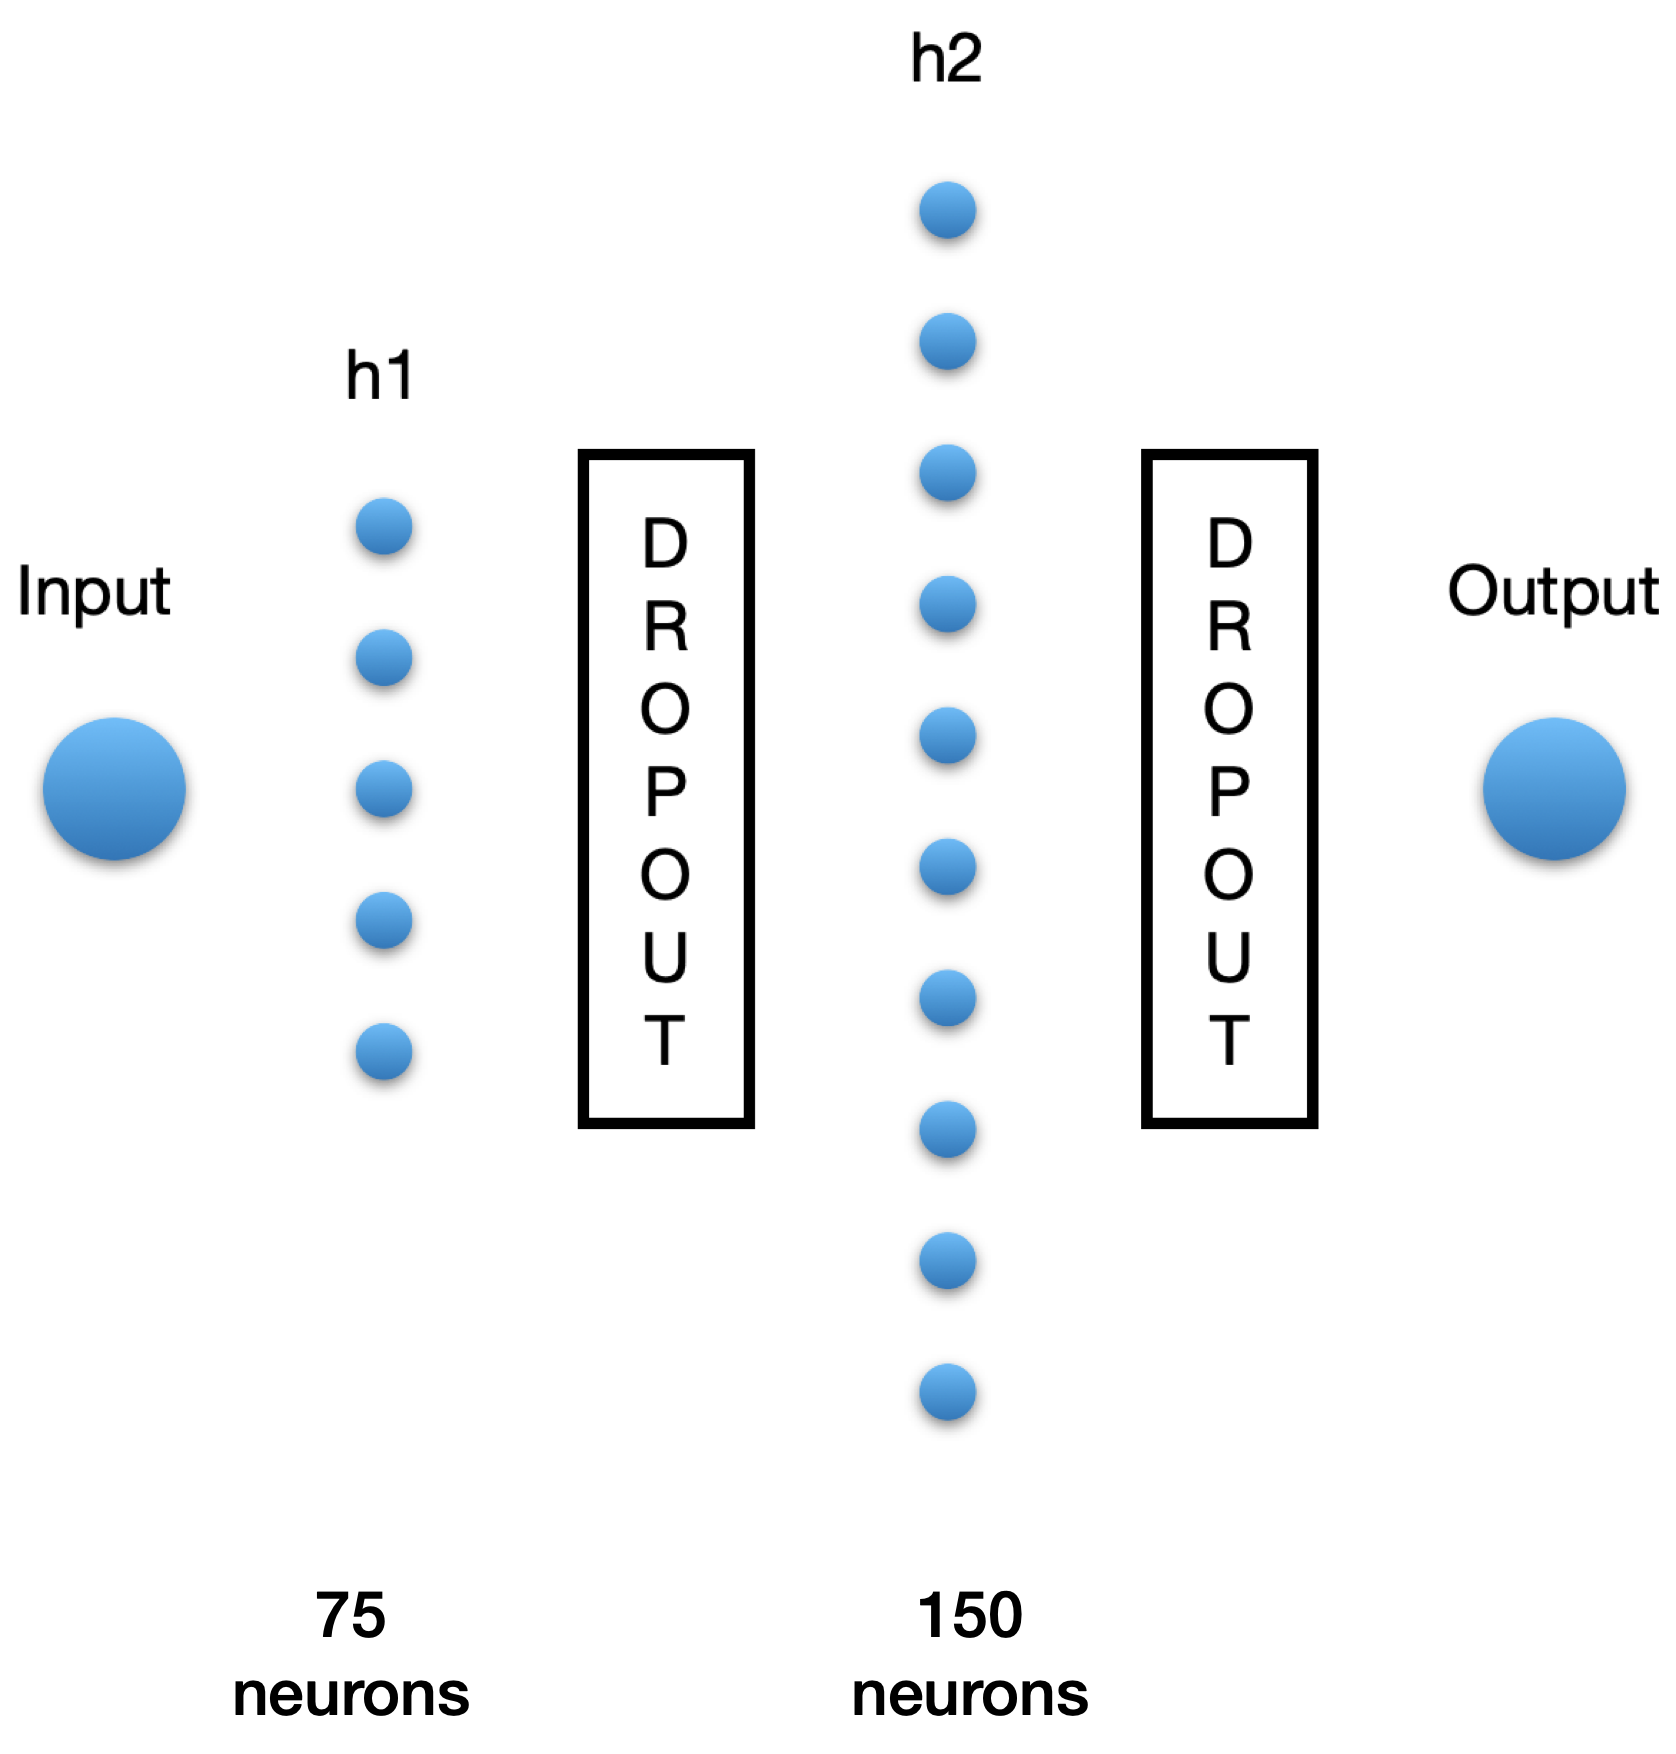
\includegraphics[width=0.5\textwidth]{Images/Regression_network.png}
    \caption{Final network for the regression task. The activation function is the rectified linear unit.}
    \label{fig:reg_net}
\end{figure}
The grid search lead to the parameters in Table \ref{tab:reg_par}.
\begin{table}[h]
    \centering
    \begin{tabular}{cccccc} \hline
        Dropout & Epochs & Learning rate & Optimizer & Regularization & Hidden units \\ \hline
        $0.023$ & $400$  & $0.0004$      & Adam      & $0$            & $75$
    \end{tabular}
    \caption{Optimal parameters for the regression task.}
    \label{tab:reg_par}
\end{table}

We can finally test our network on the test set. We stress that the splitting of test and training test was not optimal, 
since we have two missing intervals in the input space. However, it is not always possible to have the full dataset, and
we so pushed for the generalization capabilities of the network, using in particular the regularization which mitigates the 
overfitting problem. 
We can see from Figure \ref{fig:reg_pred} that the first maximum is well predicted by the model, while the second one is cut.
\begin{figure}[h]
    \centering
    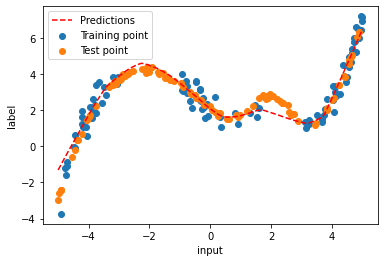
\includegraphics[width=0.6\textwidth]{Images/regression_pred.png}
    \caption{Data points with the model prediction. We can see that the model is able to reproduce the first maximum, but cuts the 
        second.}
    \label{fig:reg_pred}
\end{figure}
To gain a better insight in why we have this behavior we investigate the weight histograms and the activation profiles
of the network.
From Figure \ref{fig:reg_weights} we can not really extract useful information.
It is instead really important to observe the activation profiles, in which we plot on a $3d$ plot the activation profile
wrt the input space for some of the neurons. In the first layer, presented in Figure \ref{fig:reg_h1}, we can see that the network strongly divide the right and left
part of the input space, as we can expect since the behavior in the two regions is completely different. The second layer 
profile, in Figure \ref{fig:reg_h2}, shows instead a profile more similar to the output of the network. We can see that some neurons actually have located the second maximum of the 
function, but on average it is hidden, as we can see from the thick red line.
\begin{figure}[h]
    \centering
    \begin{minipage}[t]{0.48\textwidth}
        \centering
        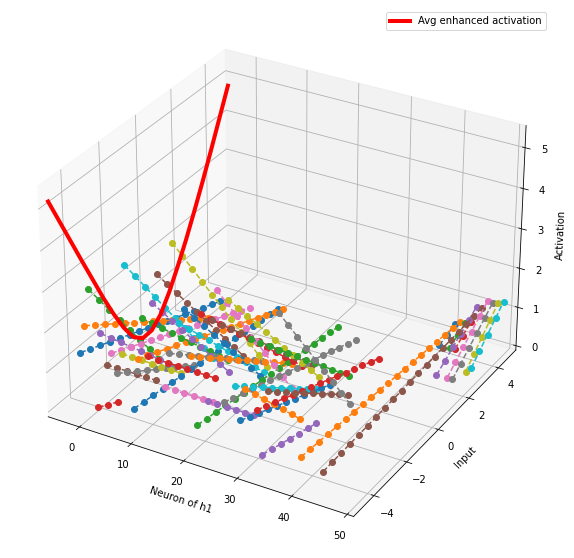
\includegraphics[width=0.98\textwidth]{Images/reg_h1.png}
        \caption{Activation profile of the first hidden layer. In thick red we can see the average of the profiles of the 
            neurons, multiplied by a constant to better catch the behavior. It is clear that this layer is able to understand
            if the input is on the left or right side of the input domain.}
        \label{fig:reg_h1}
    \end{minipage}\hfill
    \begin{minipage}[t]{0.48\textwidth}
        \centering
        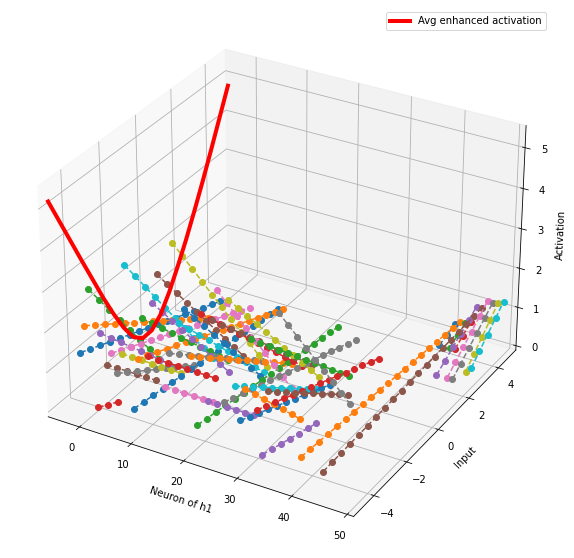
\includegraphics[width=0.98\textwidth]{Images/reg_h1.png}
        \caption{Activation profile of the second hidden layer. The average enhanced activation is defined as in Figure \ref{fig:reg_h1}.
            We can notice from this plot that the first maximum is well represented, while the second one is cut even if some of the
            neurons actually are particularly active in that interval.}
        \label{fig:reg_h2}
    \end{minipage}
\end{figure}

We can so conclude that we had an acceptable result in the regression task, even if not perfect.